% \documentclass{IEEEtran} 
\documentclass{IEEEconf} 
\usepackage{url}
% \usepackage{hyperref}
\usepackage{amssymb,amsmath}
\usepackage{pdfpages}
\usepackage{graphicx}

\title{No solution? Clustering to Evaluate Multiple Imputation } 
\author{Anthony S. Chapman, Dr Steven Turner, Dr Wei Pang, Dr Lorna Aucott} 
\begin{document} 
	\maketitle{} 

% Glad I could help. You already have a quarter of a paper. 
% Some initial comments:
% Personally, I would do the discussion before the conclusion, or incorporate the two together as Discussion and Conclusion. Remember - don't use colloquial language.
% Also, you want to head a section as The Problem to make it abundantly clear what it is. You need to lead them by the nose. You must always explain what you are going to tell them, tell them what you are going to tell them, then tell them what you have told them to get the message across -subtly, of course. Expand Acronyms the first time you use them. Also, explain everything if you want the paper to appeal to a wider audience. If you write for an audience who understand all the language, great for them, but if you want to refer to it later for a different audience, better to make it super clear and lead them by the hand.

% Anyway - you are off and running. Good luck - you'll have three papers in no time at all.

% There is nothing to easily compare different imputation techniques, post researches haven't got computing background... (need a way to formally say that statement, maybe number of disciplines VS computing?? ) 

	\abstract{Blah}

	\section{Introduction} % (fold)
	\label{sec:introduction}
		Introduce the paper not the problem.
	% section introduction (end)

	\section{Background} % (fold)
	\label{sec:background}

	In this section we introduce some key concepts and why they are needed. 

		\subsection{Missing Data} % (fold)
		\label{sub:missing_data}
		Like many other scientists, from all disciplines, we encountered datasets with missing values within them\cite{bigData}. The amount of missingness on some of these datasets was as high as 75\% of all records having one or more values missing. Before any analysis can be carried out, we need to decide on what to do with the datasets. The first options is to ignore any missing values and carry out the analysis on the subset consisting of all records with no missing values (complete case analysis). The second option is to replace (impute) any missing values with what is likely to be there correct values.

		Looking through some systematic reviews of cohort studies \cite{systematic1,systematic2,systematic3} we were able to see how hundreds of different studies dealt with missing data. The majority (circa 70\%) seems to carry out complete case analysis, and some (circa 25\%) don't mention whether there were any missing values or what they did if there were. \textcolor{red}{(Theory about most data possible for better analysis)} In our case, this would mean only being able to use 30\% of the data available. Although ignoring missing values seems to be the norm, the systematic reviews also show studies which use imputation methods before their analysis to deal with the missinng values. Imputation has been shown to be useful\cite{impact} but it should not be taken lightly, \cite{systematic1,systematic2} have shown 9\% and 6\% (respectively) of the studies they reviewed used imputation methods that are known to produce biased results.
		% subsection missing_data (end)

		\subsection{Imputation} % (fold)
		\label{sub:imputation}
		
		Once it was decided that we would rather impute datasets instead of conducting complete case analyses, we set about finding the best imputation techniques. We decided to use the statistical computing software R \cite{r} for any analysis and after plenty of searching settled with a package called MICE \cite{mice}. Although it seems to be a good imputation package, how are we sure that this imputation methods (or any) will enhance our data for better analytical results. Even if this method has been proven to work on another daatset, it is no indication that it will work on any other. 

		\textcolor{red}{maybe explain multiple imputation...}

		In order to check whether the imputation method works on a given dataset, one can first apply the method to a benchmark dataset and analyse the effects of such an action. For this process to imply the effects of the method on the given dataset, the benchmark must behave as close as possible to the dataset. Unfortunately, it is often very difficult and time consuming to find such a benchmark. It would be almost impossible to find a benchmark which could also be used for any given dataset. Thus, we felt that benchmark datasets should also be specific to the given dataset. Once could create a benchmark by analysing the way data is missing in the dataset and applying it to a dataset which is complete. The best complete dataset to mimic the original behaviour could be a complete cases dataset extracted from the original dataset. 
		% subsection imputation (end)

		\subsection{Clustering} % (fold)
		\label{sub:clustering}
		
		The next challenge will be to interpret the effect of imputing a dataset with any given imputation method. Measure theory and clustering provide us with good starting points on achieving this, measure theory related to systematic ways in which to assign numbers to suitable members of a group, this way one can give a sense of distance in a less conventional manner (for example, what is the distance between record 5 in a dataset and the average record in the same dataset, note the dataset could include non-numerical variable). Clustering is an unsupervised computation method which takes a group of items and puts them into smaller groups according to their characteristics. The idea being, all items that behave similarly will be put into one group and all other items will be in other groups.
		% subsection clustering (end)

		% Talk about systematic review papers that review cohort studies and how they deal with missing values \cite{systematic1,systematic2}
		% \cite{systematic1} 66\% complete case analysis (ignore missing data), 9\% used imputation methods that are known to produce biased results
		% \cite{systematic2} 62.5\% didn't report whether any missing data was encountered or how they delt with it, 6\% used impuatation methods that are known to produce biased results
		% \cite{systematic3} Argument  about the effects of imputation vs complete-case analysis - acknowledges missing data is everywhere

		% Talk about something \cite{epi1}
		% \cite{bigData}
		% No existing solution
		% Data collection has been increasing 
		% Missing data is inevitable (human and computing reasons, i.e. people not putting it in or computer corrupting it, )
		% Non-computing people either imputate willy-neely or ignore missing data - need to use as much data as you can. (Ask Graham about theory about using as much data as possible for better analysis)
		% Many imputation algorithms out there with many parameters, which is best? 
		% Need 

		% You can look at any cohort study you chose Anthony!  What might be more meaningful is to look at a number of systematic reviews on a topic and then look at the completeness of data within each review.  This will give you 4-5 references which encompass up to 100 original papers.  I attach a SR on asthma aetiology.  You could look for SRs on other non-communicable diseases in  childhood (and ideally the ones you are going to look at, eg obesity, epilepsy, ADHD and diabetes).

	% section background (end)

	\section{The Problems} % (fold)
	\label{sec:the_problems}
	When working with raw routinely acquired data, one of the first problems a researcher will have to overcome is how to deal with missing values \cite{rountine-missing}. With so much data being collected daily \cite{bigData}, it is no wonder that some of the data may become corrupt within the process, from gathering it to it being stored. These data corruptions may happen due to human error, computational inefficiency or other unforeseen circumstances \cite{reason}. Missing values in a dataset create an array of questions that need to be answered, namely, will it affect the results from any analysis, what can be done with records with missing values, if a solution to another dataset with missing values is found, will it work on another and lastly, if more than one solution is found, which one is the best for a specific dataset. We now discuss some of these problem and provide possible solutions.

		\subsection{Incompleteness / Missing Values} % (fold)
		\label{sub:incompleteness}
			When analysing data at it's most raw form, the amount of missing values in datasets are at their highest.
			% This problem is at it's biggest the closest one gets to the raw data, ie the data stored at it's purest form.
			Although there are ways to combat missing data, such as mean-value imputation or multiple imputation \cite{missing1,missing2,missing3}, many researchers whom may not be computationally or statistically confident would rather ignore any records with missing values \cite{epi1,systematic1,systematic2,systematic3}. As an example, in \cite{epi1}, the authors decided to use 2,758 records for analysis out of the possible 44,261 mainly due to missing data, this is a mere 6.2\% out of the records available. There must be a way for even non-computing or non-statistical researchers to benefit from the tools available. 
			\subsubsection{Possible Solution: Imputation} % (fold)
			\label{sub:possible_solution}
				Imputation is the process of replacing missing values with substituted values, one has to be careful when imputing data as there are many techniques (default value, mean value and multiple imputation just to name a few \cite{gelman2007data}) and using them without care will lead to erroneous data analysis \cite{careful}. By creating a user-friendly system with clear guidelines on how to impute data and some explanation on how it works, we believe that researchers whom would normally ignore data with missing values will be more likely to use more of their data through imputation, thus improving the quality and credibly of their analysis.
			% subsection possible_solution (end)
		% subsection incompleteness (end)
		\subsection{Will it work on my data./Does it work for all datasets.} % (fold)
		\label{sub:will_it_work_on_my_data}
			After deciding that imputation is beneficial to the study, the next step will be to find an imputation method for the dataset. Some good starting points may be Muliple Imputation by Chained Equations (MICE \cite{mice}) using the computational language R \cite{r} or the Impute Missing Values function in the statistical software SPSS \cite{spss}. The problem is, how does one know if the imputed values are representative to the truth, how does one know whether record 2,754 column 5 is ``42'' or not after applying the imputation method.

			Even if the imputation method has been proven to work on someone else's dataset such as \cite{compare}, it is no indication it will work for any other dataset. This is due to the complex nature that missing data is created, for example there might be a relationship between one missing value and another one. 

			In order to test whether an imputation method works on any specific dataset, one needs something to compare the results to a benchmark. Then an analysis can be carried out to assess the effects of the imputation. Unfortunately, it is very difficult to find a complete dataset which contains the same characteristics as any another dataset, there will always be differences. 
			\subsubsection{Possible Solution: Testing your own data} % (fold)
			\label{sub:possible_solution}
				The proposed solution is to create clone datasets by analysing the missingness characteristics from a given dataset and applying them to a new dataset created by only keeping the complete records. We can therefore create artificial mini datasets which behave in the same manner as the original dataset. In this manner we will be left with an original dataset, a subset consisting of only the complete records (the benchmark) and artificially incomplete datasets created from the complete records with the characteristics from the original. 

				We then have a benchmark and a testing dataset that is as close to your original dataset as any dataset can be. The idea being that if the imputation method works on the testing datasets, then it will work on the original, and we can test whether imputation is successful by comparing to the benchmark. 
			% subsection possible_solution (end)
		% subsection will_it_work_on_my_data_(end)
		\subsection{Which imputation is best for me} % (fold)
		\label{sub:which_imputation_is_best_for_me}
			The following problem applies to researchers, even those computationally competent, who wish to know whether one imputation method is better than another. There is nothing to easily compare results from different imputation methods or same imputation methods with slightly different parameters. The main problem arises when one tries to compare the outcomes from one method to another, here an adequate analogy would be to compare imputation method A to method B would be like comparing chocolate with a bicycle; the outcomes might not be comparable. 

			There should be a program that can take different imputation methods and output something that can be compared to the output from another imputation methods. Having to do this is hard enough if you have a computing degree, so it is essential that something can be created that everyone can use. 
			\subsubsection{Possible Solution: Comparing Imputation} % (fold)
			\label{sub:possible_solution}
				In order for a researcher to be able to compare different imputation techniques on their own datasets, the outcomes of the techniques need to ``talk the same language''. Creating a program that takes in a dataset and any imputation method and outputs a standardised efficiency classification we will be able to compare different imputation methods on the same dataset using this standardised efficiency classification. Thus every researcher will be able to compare different imputation methods without having to understand the individual imputation technique outputs.
			% subsection possible_solution (end)
		% subsection which_imputation_is_best_for_me (end)
	% section the_problems (end)

 

	\section{Proposed Framework} % (fold)
	\label{sec:proposed_framework}
		\textbf{The idea:} The underlying concept is to first create a benchmark dataset from the complete records, then create artificially missing datasets, which represent the original dataset, out of the benchmark by mimicking the original dataset. We achieve this by analysing how data is missing and create testing datasets by imposing the same missingness into the benchmark. We would then impute the artificially missing datasets and analyse how far they have travelled from the benchmark. We can check how far imputation has taken the datasets from the benchmark by clustering the benchmark and the testing datasets. Like this we will be able to see the effects of any imputation technique on any dataset. 
		\\
		\indent \textbf{Pre-requisite:}
		In order to evaluate an imputed dataset, one has to first have a dataset with missing values and an imputation method. At this stage, any imputation method can be used, this accommodates the ability to compare different imputation methods on the same dataset to evaluate the best one. Similarly, one can apply the same imputation methods to the dataset multiple times by changing the imputation parameters, thus finding the optimal imputation. We will caal the dataset $O$ and imputation method $imp(x)$, were $x$ is any incomplete dataset.
		\\
		\indent \textbf{Stage 1: Extracting Benchmark}
		Firstly we need to create a benchmark dataset by extracting all the complete records from $O$, we call this benchmark dataset $CC$ for Complete Cases. We then analysis $O$ and find it's missingness characteristics, this will be used to create replicas later in the process. Notice that $ CC \subset O$ 
		\begin{figure}[!ht]
			\caption{Stage 1}
			\centering
			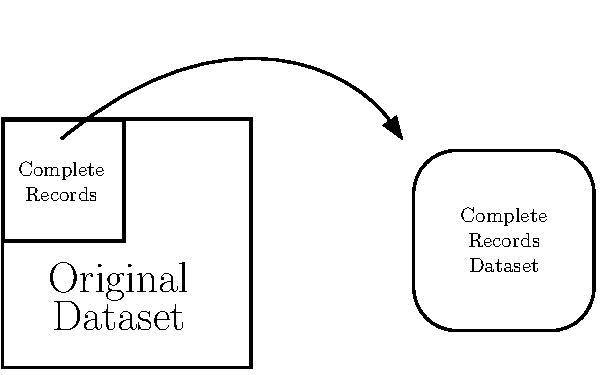
\includegraphics[width=0.35\textwidth]{stage1.pdf}
		\end{figure}
		\\
		\indent \textbf{Stage 2: Create Dummy Datasets}
		Next, we create $n$ artificially incomplete datasets, called $artMiss.i$ where $i$ is a number from 1 to $n$ by applying the missingness characteristics from $O$ to $CC$ $n$ times. It is important to apply the missingness in a manner that treats each $artMiss.i$ separately, this way we can test the imputation more robustly. Thus we now have a benchmark dataset $CC$, and $n$ artificial datasets with missing data which follow the same structure as the original dataset.
		\begin{figure}[!ht]
			\caption{Stage 2}
			\centering
			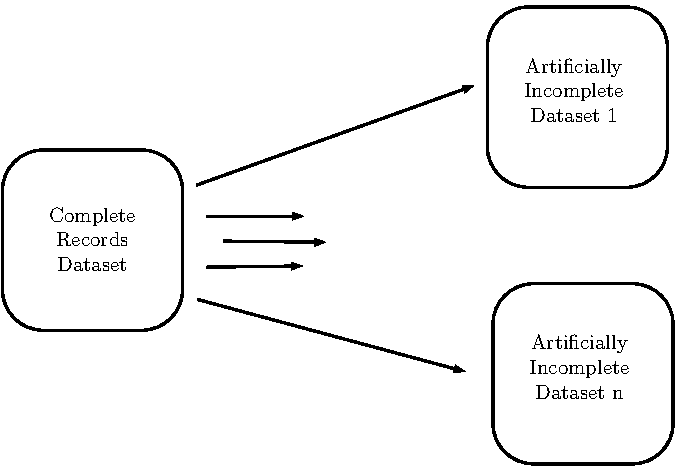
\includegraphics[width=0.35\textwidth]{stage22.pdf}
		\end{figure}
		\\
		\indent \textbf{Stage 3: Impute Dummy Datasets}
		The next step will be to impute all $artMiss.i$ using the chosen imputation method, it is very important to apply exactly the same procedure (same imputation with the same parameters)to all datasets in order to have reliable results, the imputation process must be deterministic. This will create $n$ artificially complete (imputed) datasets, called $artComp.i$ where $i$ is a number from 1 to $n$. 
		\begin{figure}[!ht]
			\caption{Stage 3}
			\centering
			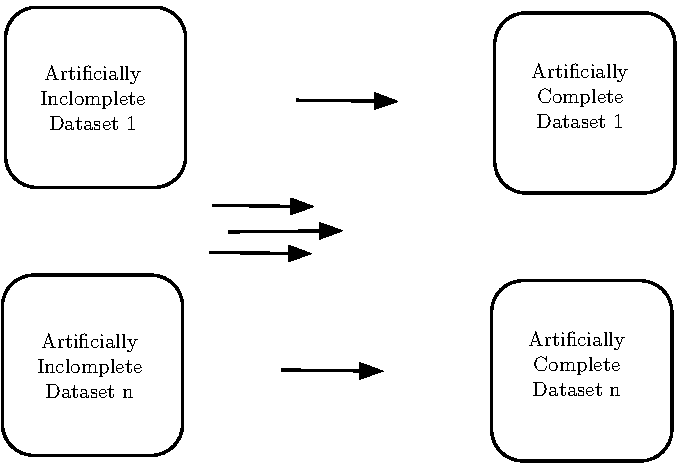
\includegraphics[width=0.35\textwidth]{stage3-2.pdf}
		\end{figure}
		\\
		\indent \textbf{Stage 4: Cluster all Datasets}
		In order to evaluate the effect of an imputation method, we will use clustering techniques and measure theory to find the distance between all $artComp.i$ and $CC$. By finding the distance between sets of cluster, we can see how close (or far) an imputation method has taken each $artMiss.i$ from the true values (the benchmark $CC$). We will now be able to compare the effect of different imputation methods and evaluate each one.

		Thus we need to cluster our benchmark dataset $CC$ and all imputed datasets $artComp.i$, we will call $clustCC$ the clustering of $CC$ and $clust.i$ will be all clustered $artComp.i$. Note that as with imputing all datasets we need to make sure the same clustering method with the same parameters in being used. This way we can accurately calculate the distances between the datasets. Similarly to the imputation process, for this to work, the clustering process must be deterministic.
		% we will combine all artComp.i into one dataset by averaging the information. All imputed variables will create one average variable and all the results that were there originally will be the same. By doing this will be able to comfortably compare this master artificially complete dataset with the benchmark CC. 
		\begin{figure}[!ht]
			\caption{Stage 4}
			\centering
			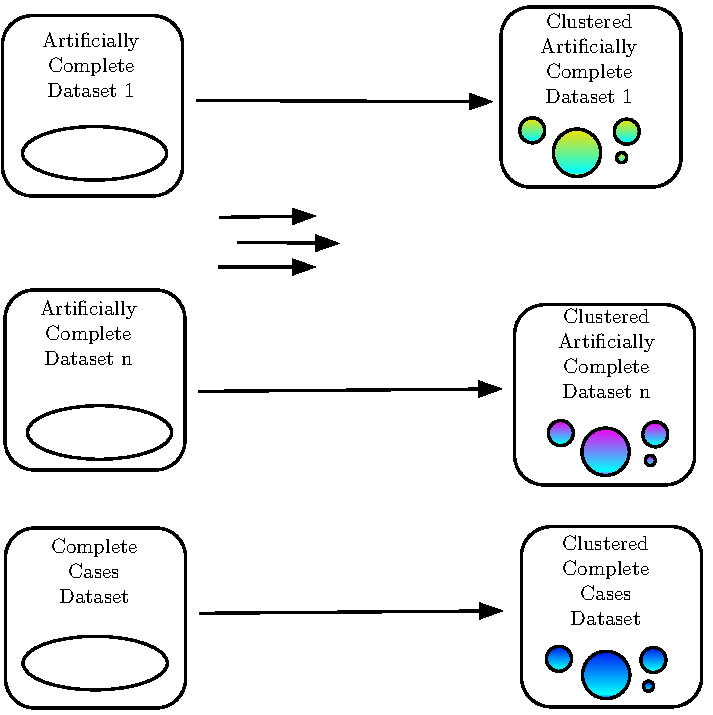
\includegraphics[width=0.35\textwidth]{stage4-2.pdf}
		\end{figure}
		\\
		\indent \textbf{Stage 5: Distance Between Dummies and Benchmark}
		Finally, we will need to calculate the distance between all $clust.i$ and $clustCC$. This will indicate the effect of imputing an incomplete dataset by finding the distance between the clustering of the imputed datasets ($clust.i)$ and the clustering of our benchmark ($clustCC$). The system should output an efficiency indicator to show how far away all $clust.i$ are from $clustCC$, this will be how we judge whether an imputation method gives correct values or not. 

		Whether the final output describes a successful or efficient imputation method will be subjective. Each researcher will have to decide whether the imputed values are close enough to represent the truth or whether they are too far to provide fair results from any type of analysis. 
		% We then need to compare how far away the artComp.i clustering have gone from the CC's clustering. This can be done by comparing the clustering characteristics such as their medoids, cluster widths, and how sparse the data points are. It will be the researcher's decision on whether the imputation be classed as successful or not according to the output. 
		% It would be beneficial for the output to have a scale in which the researcher will be able to judge the imputation methods (ie. 40\% efficient of it travelled 15\% from benchmark).
		\begin{figure}[!ht]
			\caption{Stage 5}
			\centering
			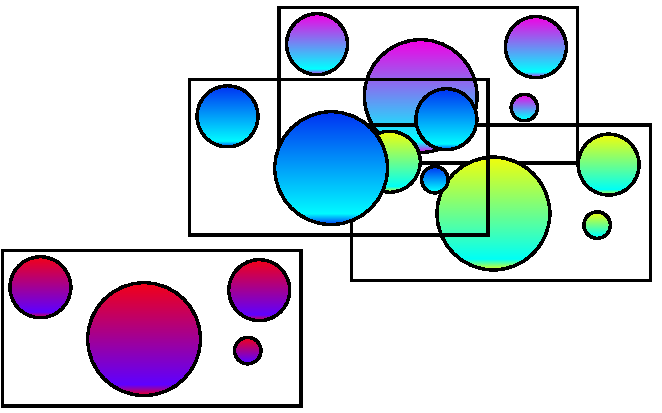
\includegraphics[width=0.35\textwidth]{stage5-2.pdf}
		\end{figure}
		\\
	% section proposed_framework (end)

	\section{Discussion} % (fold)
	\label{sec:discussion}
		It would be beneficial for the output to have a scale in which the researcher will be able to judge the imputation methods (ie. 40\% efficient of it travelled 15\% from benchmark). These will be discussed at a later date
		
		Ways to compute the distance between two clusterings (not individual clusters) 
		
		We need a reference point to judge whether the imputation is good or not, mean imputation as a reference point.

		Distance measure - could also use modelling to create models of each dataset and compare the results 


	% section discussion (end)

	\section{Conclusion} % (fold)
	\label{sec:conclusion}
		
	% section conclusion (end)



	\bibliographystyle{plain}
	\bibliography{../papers}

\end{document}

We could also check this by creating models of both the benchmark and the imputed datasets. 

The first step will be to analyse the original dataset to find the missing value characteristics. We then great a dataset out of the original one by deleting all the records with missing values in it. The next step will be to create n amount of artificial datasets 


	\section{Possible Solutions } % (fold)
	\label{sec:possible_solutions_}
		\subsection{Incompleteness} % (fold)
		\label{sub:incompleteness}
			Imputation will create values where there were non before, one has to be careful when imputing data as there are many techniques (default value, mean value and multiple imputation just to name a few) as using them without care will lead to erroneous data \cite{careful}. By creating a user-friendly program with clear guidelines on how to use it and some explanation on how it works, we believe that researchers whom would normally ignore data with missing values will be more likely to use more of their data through imputation.
		% subsection incompleteness (end)
		\subsection{Testing your own dataset} % (fold)
		\label{sub:testing_your_own_dataset}
			In order to test how well an imputation technique, such as MICE, one needs to be able to compare the effects of the imputation method to a benchmark, we propose creating a benchmark from the users own dataset. By analysing the missing data characteristics, extracting the subset of complete data from the dataset and then replicating the same dataset onto the subset, we are able to create artificial mini datasets which behave as the original one except now we have a benchmark to compare the effects of imputation. 

		% Use your own level or missingness as a benchmark and create mini-me's as bench-mark. You are the closest thing to yourself. 
		% Group theory stuff, multidimensional-mixed data distance measurements, Gower, medoids, widths and dissimilarities.

		% Just because it worked on someone else, doesn't mean it works for you, cite papers who test specific datasets. 
		% subsection testing_your_own_dataset (end)
		\subsection{Comparing imputations} % (fold)
		\label{sub:comparing_imputations}
			In order for a researcher to be able to compare different imputation techniques on their own datasets, the outcomes of the techniques need to ``talk the same language''. By having a program that takes a dataset and imputation pair and then outputs the efficiency of the imputation, one is able to compare these outputs with ease and without having to understand the individual imputation technique outputs. 

			% Will now be able to compare different imputations on your own dataset with ``normalised '' results for comparison. 
		% subsection comparing_imputations (end)
	% section possible_solutions_ (end)

	\section{The Framework} % (fold)
	\label{sec:the_framework}

		\begin{figure}[!ht]
			\caption{Framework flowchart}
			\centering
			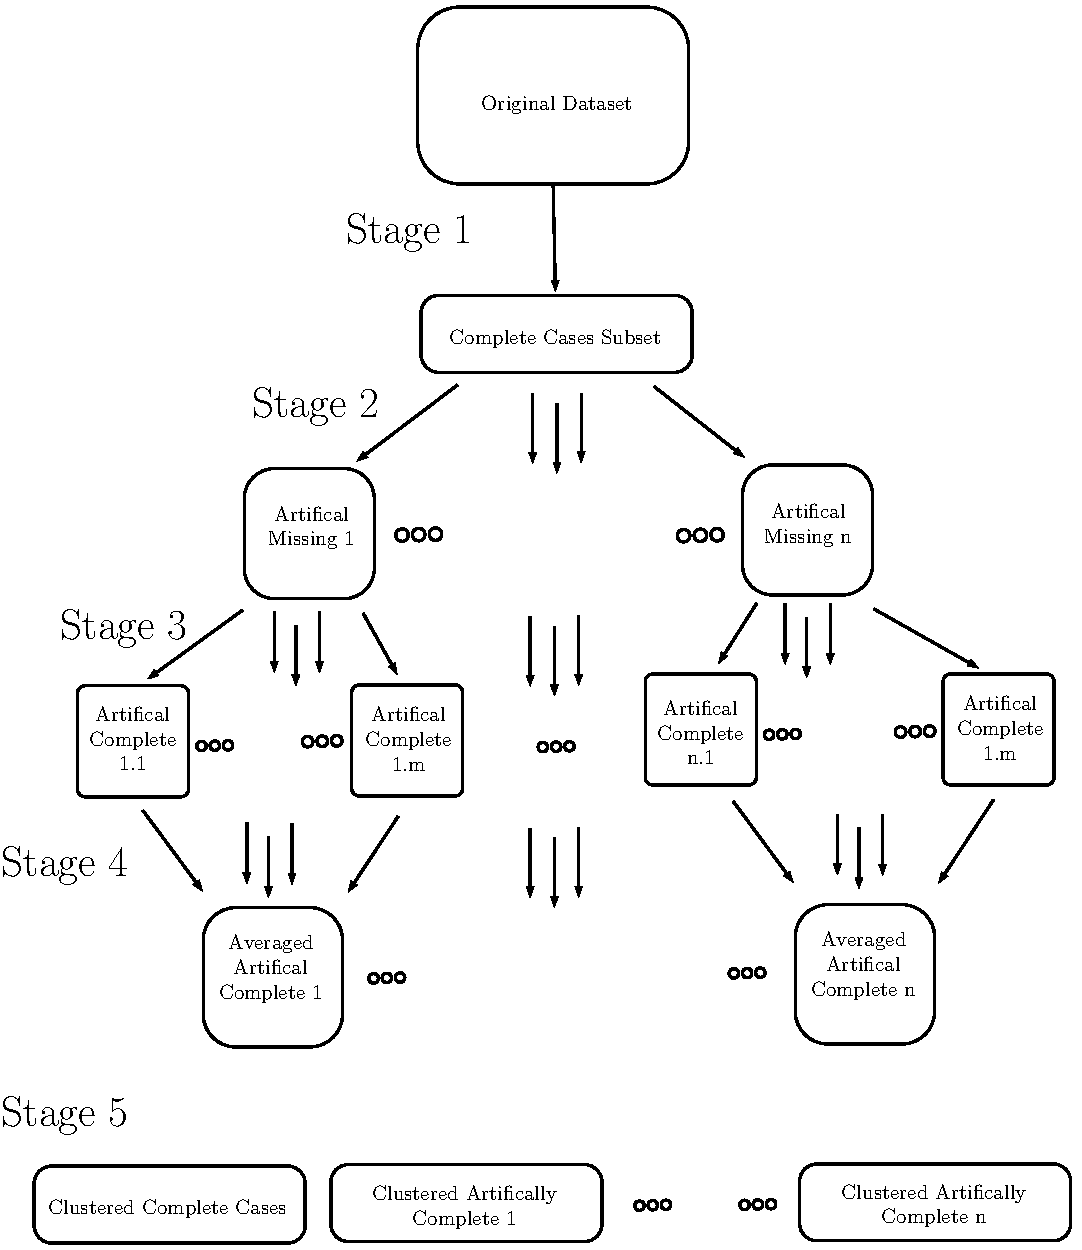
\includegraphics[width=0.5\textwidth]{diagram.pdf}
		\end{figure}
		The process is as follows: Using a dataset with missing values, call this ``OD'', for original dataset, and an imputation technique, call this ``Imp'', you first analyse the missingness characteristics of ``OD'' to in order to apply them later. Then, create a new dataset by deleting any record from ``OD'', call this "CC", for complete cases. Using the missingness characteristics, we create more da

		The proposed framework is as follows: In order to assess the effects of any imputation technique, the program will need a dataset with missing values, called ``D'', and an imputation method, called ``I''. Then the function ``I(x)'' is a function that takes a data with missing values and outputs an imputed dataset. 

		Specify dataset (O) and imputation method (I)
		Analyse dataset to obtain the missing characteristics
		Create subset of dataset with only complete cases (C)
		Apply missing characteristics to create n individual datasets out of C, called ($ArtM_{1}, ArtM_{2}...ArtM_{n}$)
		Impute all $Art_{n}$ to created artificially complete datasets $ArtC_{n}$
		Apply clustering algorithm to C and all $ArtC_{n}$ to create $ClustC$ and $ClustArt_{n}$
		Average clustering outcomes from all $ClusArt_{n}$ and compare to $ClustC$
		Analyse how far the average of all $ClusArt_{n}$ have gone from $ClustC$
		Normalise the distance to give a percentage of goodness for the user.
	% section the_framework (end)

	\section{Conclusion} % (fold)
	\label{sec:conclusion}
	It's better to use all the data you can but can't blindly imputation. This framework indicates whether your data 
	% section conclusion (end)

	\section{Discussion} % (fold)
	\label{sec:discussion}
	Working on implementing this, ClEMI, any researcher regardless their computing ability will be able to use it. 
	% section discussion (end)

	A receiver operated characteristic curve will be used to determine the CRL z score with best sensitivity and specificity for outcomes. For asthma severity (measured on ordinal scale of 1-5 and based on treatments prescribed) we will use ordinal logistic regression.



You can look at any cohort study you chose Anthony!  What might be more meaningful is to look at a number of systematic reviews on a topic and then look at the completeness of data within each review.  This will give you 4-5 references which encompass up to 100 original papers.  I attach a SR on asthma aetiology.  You could look for SRs on other non-communicable diseases in  childhood (and ideally the ones you are going to look at, eg obesity, epilepsy, ADHD and diabetes).
 
Best wishes
Steve